\documentclass[nobib,notoc,twoside,symmetric]{tufte-book}
\setcounter{tocdepth}{4}
\setcounter{secnumdepth}{4}

\usepackage{marginfix}
%to fix margins
\usepackage{multicol}
%for two-column.
\usepackage{CJKutf8}
%for mandarin

%\usepackage{scrextend} 
%\changefontsizes[11pt]{12pt}

\renewcommand{\footnotesize}{\small}

\geometry{a4paper,landscape,inner=30mm,top=15mm,bottom=10mm,headsep=\baselineskip,textwidth=170mm,marginparsep=8mm,marginparwidth=80mm,textheight=170mm,headheight=\baselineskip}

%\geometry{showframe}% for debugging purposes -- displays the margins

%\usepackage{stmaryrd}
%\usepackage{fontawesome}

\usepackage{amsmath,amsthm,amssymb,amsfonts}
\theoremstyle{definition}
\newtheorem{theorem}{Theorem}[section]
\newtheorem*{theorem*}{Theorem}
\newtheorem{corollary}[theorem]{Corollary}
\newtheorem{lemma}[theorem]{Lemma} 
\newtheorem{proposition}[theorem]{Proposition}
\newtheorem{conj}[theorem]{Conjecture}
\newtheorem{defn}[theorem]{Definition}
\newtheorem{fact}[theorem]{Fact} 
\newtheorem{example}[theorem]{Example} 
\newtheorem{examples}[theorem]{Examples}
\newtheorem{example*}[theorem]{Example*}
\newtheorem{examples*}[theorem]{Examples*}
\newtheorem{remark}[theorem]{Remark}
\newtheorem{remark*}[theorem]{Remark*}
\newtheorem{question}[theorem]{Question}
\newtheorem{assumption}[theorem]{Assumption}
\newtheorem{conjecture}[theorem]{Conjecture}
\newtheorem{convention}[theorem]{Convention}
\newtheorem{justification}[theorem]{Justification} 
\newtheorem{construction}[theorem]{Construction}
\newtheorem{rem}[theorem]{Reminder}
\newtheorem{intuition}[theorem]{Intuition}
\newtheorem{term}[theorem]{Terminology}
\newtheorem{scholium}[theorem]{Scholium}
\newtheorem{requirement}[theorem]{Requirement}
\newtheorem{notation}[theorem]{Notation}
\newtheorem{refinement}[theorem]{Refinement}
\newtheorem{thesis}[theorem]{Thesis}

%for fonts
\usepackage{newpxtext}
%\usepackage[fracspacing]{newpxmath}
\linespread{1.05}

\usepackage{tikz-cd}
\usepackage{macros/tikzfig}
\usepackage{macros/quiver}
\input{macros/thesis.tikzstyles}

% Set up the images/graphics package
\usepackage{graphicx}
\setkeys{Gin}{width=\linewidth,totalheight=\textheight,keepaspectratio}
\graphicspath{{graphics/}}

\title{String diagrams for text}
\author[V.W.]{Vincent Wang-Ma\'{s}cianica}
\date{\today}

% The following package makes prettier tables.  We're all about the bling!
\usepackage{booktabs}

% The units package provides nice, non-stacked fractions and better spacing
% for units.
\usepackage{units}

% The fancyvrb package lets us customize the formatting of verbatim
% environments.  We use a slightly smaller font.
\usepackage{fancyvrb}
\fvset{fontsize=\normalsize}

% Small sections of multiple columns
\usepackage{multicol}

% Squares
\usepackage{stix}

% Provides paragraphs of dummy text
\usepackage{lipsum}

% These commands are used to pretty-print LaTeX commands
\newcommand{\doccmd}[1]{\texttt{\textbackslash#1}}% command name -- adds backslash automatically
\newcommand{\docopt}[1]{\ensuremath{\langle}\textrm{\textit{#1}}\ensuremath{\rangle}}% optional command argument
\newcommand{\docarg}[1]{\textrm{\textit{#1}}}% (required) command argument
\newenvironment{docspec}{\begin{quote}\noindent}{\end{quote}}% command specification environment
\newcommand{\docenv}[1]{\textsf{#1}}% environment name
\newcommand{\docpkg}[1]{\texttt{#1}}% package name
\newcommand{\doccls}[1]{\texttt{#1}}% document class name
\newcommand{\docclsopt}[1]{\texttt{#1}}% document class option name

\usepackage{bussproofs}

\usepackage{xcolor}
\usepackage{xspace}
\def\bB{\begin{color}{blue}}
\def\bO{\begin{color}{orange}}
\def\bG{\begin{color}{green}}
\def\bM{\begin{color}{magenta}}
\def\e{\end{color}\xspace}

%For chesspieces
\usepackage{skak}

%For Brakets
\usepackage{physics}

\usepackage{xspace} 
%\usepackage{enumerate}
\usepackage{color} 
\def\bR{\begin{color}{red}}
\def\bB{\begin{color}{blue}}
\def\e{\end{color}\xspace}

%\usepackage{tocloft}
%\cftsetindents{section}{0em}{2em}
%\cftsetindents{subsection}{0em}{2em}
%\renewcommand\cfttoctitlefont{\hfill\Large\bfseries}
%\renewcommand\cftaftertoctitle{\hfill\mbox{}}

\begin{document}

\maketitle% this prints the handout title, author, and date

%\begin{fullwidth}
%\begin{multicols}{2}
\tableofcontents\marginnote{(Acknowledgements will go in a margin note here.)}
%\end{multicols}
%\end{fullwidth}


\chapter{Sketches in iconic semantics}\label{chapter:contrel}
How to reason formally with and about pictorial iconic representations as a semantics of natural language.
\clearpage
\newpage
\section{Continuous Relations for iconic semantics}\label{sec:contrelintro}

\begin{figure}[h!]
\centering
\[\resizebox{\textwidth}{!}{\tikzfig{topology/conduitmetaphor}}\]
\caption{Sometimes it is very helpful to illustrate concepts using iconic representations in cartoons. For instance in the \emph{conduit metaphor} \citep{reddyConduitMetaphorCase}, \texttt{words} are considered \emph{containers} for \texttt{ideas}, and \texttt{communication} is considered a \emph{conduit} along which those containers are sent.}
\end{figure}

The aim of this chapter is to give us a formal setting in which we can paint pictures with words. More verbosely, to formalise cartoon doodles like the one above in a symmetric monoidal category so that we can give semantics to text circuits in terms of graphical, iconic representations -- cartoons, in short. To do so, we introduce the category \textbf{ContRel} of \emph{continuous relations}, which are a na\"{i}ve extension of the category \textbf{Top} of topological spaces and continuous functions towards continuous relations.\\

The main reason we prefer \textbf{ContRel} to either \textbf{Rel} or \textbf{Top} for our purposes is that we can diagrammatically characterise set-indexed collections of mutually disjoint open sets as \emph{sticky-spiders}: a generalisation of spiders that interact with idempotents. We can then treat the indexing set as a collection of labels, and an indexed open set as a doodle. Notably, spiders don't exist in cartesian \textbf{Top} except for the one-point space, and the spatial structure of open sets doesn't exist in \textbf{Rel}. But there are all kinds of poorly behaved open sets even on the plane, so enter the next benefit: In \textbf{ContRel}, we can diagrammatically characterise the reals as a topological space up to homeomorphism, which gives us a diagrammatic handle on paths and homotopies, mathematical concepts that enable us to diagrammatically characterise when open sets are connected, how they might move and transform continuously in space, and when open sets are contained inside others. And once we've formalised doodles we'll be able to treat ourselves to cartoons as formal semantics for language and nobody can stop us.

\newthought{Sidenote for category theorists}

The na\"{i}ve approach I take is to observe that the preimages of functions are precisely relational converses when functions are viewed as relations, so the preimage-preserves-opens condition that defines continuous functions directly translates to the relational case. To the best of my knowledge, the study of \textbf{ContRel} is a novel contribution. I venture two potential reasons.\\

First, it is because and not despite of the na\"{i}vity of the construction. Usually, the relationship between \textbf{Rel} and \textbf{Set} is often understood in sophisticated general methods which are inappropriate in different ways. I have tried applying Kliesli machinery which generalises to "relationification" of arbitrary categories via appropriate analogs of the powerset monad to relate \textbf{Top} and \textbf{ContRel}, but it is not evident to me whether there is such a monad. The view of relations as spans of maps in the base category should work, since \textbf{Top} has pullbacks, but this makes calculation difficult and especially cumbersome when monoidal structure is involved.\\

Second, the relational nature of \textbf{ContRel} means that the category has poor exactness properties. Even if the sophisticated machinery mentioned in the first reason manages to work, relational variants of \textbf{Top} are poor candidates for any kind of serious mathematics because they lack many limits and colimits. Since we take an entirely "monoidal" approach, we are able to find and make use of the rich structure of \textbf{ContRel} with a different toolkit.

\clearpage
\newpage
\begin{fullwidth}

\section{Continuous Relations by examples}

Let's consider three topological spaces and examine the continuous relations between them. This way we can build up intuitions, and prove some tool results in the process.

The \textbf{singleton space} consists of a single point which is both open and closed. We denote this space $\bullet$. Concretely, the underlying set and topology is
\[(\{\star\} \ , \ \{\{\star\},\varnothing\})\] 
\ctikzfig{testspaces/singleton}

The \textbf{Sierpi\'{n}ski space} consists of two points, one of which (in yellow) is open, and the other (in cyan) is closed. We denote this space $\mathcal{S}$. Concretely, the underlying set and topology is:
\[\big( \{0,1\} \ , \ \{ \varnothing, \{ 1 \} , \{ 0,1\} \} \big)\]
\ctikzfig{testspaces/sierpinski}

The \textbf{unit square} has $[0,1] \times [0,1]$ as its underlying set.  Open sets are "blobs" painted with open balls. Points, lines, and bounded shapes are closed. We denote this space $\blacksquare$.
\ctikzfig{testspaces/unitsquare}
\end{fullwidth}

\newthought{$\bullet \rightarrow \bullet$:} There are two relations from the singleton to the singleton; the identity relation $\{ (\bullet,\bullet) \}$, and the empty relation $\varnothing$. Both are topological.

\newthought{$\bullet \rightarrow \mathcal{S}$:} There are four relations from the singleton to the Sierpi\'{n}ski space, corresponding to the subsets of $\mathcal{S}$. All of them are topological.


\newthought{$\mathcal{S} \rightarrow \bullet$:}
\marginnote{
\begin{example}[A noncontinuous relation]\label{ex:nontop}
The relation $\{(0,\bullet)\} \subset \mathcal{S} \times \bullet$ is not a continuous relation: the preimage of the open set $\{\bullet\}$ under this relation is the non-open set $\{0\}$.
\end{example}
}
There four candidate relations from the Sierpi\'{n}ski space to the singleton, but as we see in Example \ref{ex:nontop}, not all of them are topological.

\newthought{Now we need some abstraction.} We cannot study the continuous relations between the singleton and the unit square case by case. We discover that continuous relations out of the singleton indicate arbitrary subsets, and that continuous relations into the singleton indicate arbitrary opens.
\marginnote{
\begin{term}
Call a continuous relation $\bullet \rightarrow X^\tau$ a \textbf{state} of $X^\tau$, and a continuous relation $X^\tau \rightarrow \bullet$ a \textbf{test} of $X^\tau$.
\end{term}

\begin{proposition}\label{prop:states}
States $R: \bullet \rightarrow X^{\tau}$ correspond with subsets of $X$.
\begin{proof}
The preimage $R^\dag(U)$ of a (non-$\varnothing$) open $U \in \tau$ is $\star$ if $R(\star) \cap U$ is nonempty, and $\varnothing$ otherwise. Both $\star$ and $\varnothing$ are open in $\{\star\}^{\bullet}$. $R(\star)$ is free to specify any non-$\varnothing$ subset of $X$. The empty relation handles $\varnothing$ as an open of $X^{\tau}$.
\end{proof}
\end{proposition}

\begin{proposition}\label{prop:tests}
Tests $R: X^\tau \rightarrow \bullet$ correspond with open sets $U \in \tau$.
\begin{proof}
The preimage $R^\dag(\star)$ of $\star$ must be an open set of $X^\tau$ by definition \ref{defn:toprelation}. $R^\dag(\star)$ is free to specify any open set of $X^{\tau}$.
\end{proof}
\end{proposition}
}

\newthought{$\bullet \rightarrow \blacksquare$:} Proposition \ref{prop:states} tells us that there are as many continuous relations from the singleton to the unit square as there are subsets of the unit square.

\newthought{$\blacksquare \rightarrow \bullet$:} Proposition \ref{prop:tests} tells us that there are as many continuous relations from the unit square to the singleton as there are open sets of the unit square.

\newthought{There are 16 candidate relations $\mathcal{S} \rightarrow \mathcal{S}$ to check.} A case-by-case approach won't scale, so we could instead identify the building blocks of continuous relations with the same source and target space.

\newthought{Which relations $X^\tau \rightarrow Y^\sigma$ are always continuous?}

\newthought{The empty relation is always continuous.}
\marginnote{
    \begin{rem}[Empty relation]
    The \textbf{empty relation} $X \rightarrow Y$ relates nothing. It is defined:
    \[ \varnothing \subset X \times Y\]
    \end{rem}
}
\begin{proposition}
\label{prop:emptyrel}
\begin{proof}
The preimage of the empty relation is always $\varnothing$, which is open by definition.
\end{proof}
\end{proposition}

\newthought{Full relations are always continuous}
\marginnote{
    \begin{rem}[Full relation]
    The \textbf{full relation} $X \rightarrow Y$ relates everything to everything. It is all of $X \times Y$.
    \end{rem}
}
\begin{proposition}
\label{prop:fullrel}
\begin{proof}
The preimage of any subset of $Y$ -- open or not -- under the full relation is the whole of $X$, which is open by definition.
\end{proof}
\end{proposition}

\newthought{Full relations restricted to open sets in the domain are continuous.}
\begin{proposition}\label{prop:bowtie}
Given an open $U \subseteq X^\tau$, and an arbitrary subset $K \subset Y^\sigma$, the relation $U \times K \subseteq X \times Y$ is open.
\begin{proof}
Consider an arbitrary open set $V \in \sigma$. Either $V$ and $K$ are disjoint, or they overlap. If they are disjoint, the preimage of $V$ is $\varnothing$, which is open. If they overlap, the preimage of $V$ is $U$, which is open.
\end{proof}
\end{proposition}

\newthought{Continuous functions are always continuous.}
\begin{proposition}\label{prop:func}
If $f: X^\tau \rightarrow Y^\sigma$ is a continuous function, then it is also a continuous relation.
\begin{proof}
Functions are special cases of relations. The relational converse of a function viewed in this way is the same thing as the preimage.
\end{proof}
\end{proposition}

\newthought{The identity relation is always continuous.}
\marginnote{
    \begin{rem}[Identity relation]
    The \textbf{identity relation} $X \rightarrow X$ relates anything to itself. It is defined:
    \[ \{(x,x) : x \in X\} \subseteq X \times X\]
    \end{rem}
}
The identity relation is also the "trivial" continuous map from a space to itself, so this also follows from Proposition \ref{prop:func}.
\begin{proposition}\label{prop:idrel}
\begin{proof}
The preimage of any open set under the identity relation is itself, which is open by assumption.
\end{proof}
\end{proposition}

\newthought{Given two continuous relations $R,S : X^\tau \rightarrow Y^\sigma$, how can we combine them?}\marginnote{
\begin{rem}[Union, intersection, and ordering of relations]
Recall that relations $X \rightarrow Y$ can be viewed as subsets of $X \times Y$. So it makes sense to speak of the union and intersection of relations, and of partially ordering them by inclusion.
\end{rem}
}

\begin{proposition}\label{prop:framehom}
If $R,S: X^\tau \rightarrow Y^\sigma$ are continuous relations, so are $R \cap S$ and $R \cup S$.
\begin{proof}
Replace $\square$ with either $\cup$ or $\cap$. For any non-$\varnothing$ open $U \in \sigma$: \[(R \square S)^\dag (U) = R^\dag(U) \square S^\dag(U)\] As $R,S$ are continuous relations, $R^\dag(U),S^\dag(U) \in \tau$, so $R^\dag(U) \square S^\dag(U) = (R \square S)^\dag (U) \in \tau$. Thus $R\square S$ is also a continuous relation.
\end{proof}
\end{proposition}

\begin{corollary}\label{cor:homspace}
Continuous relations $X^\tau \rightarrow Y^\sigma$ are closed under arbitrary union and finite intersection. Hence, continuous relations $X^\tau \rightarrow Y^\sigma$ form a topological space where each continuous relation is an open set on the base space $X \times Y$, where the full relation $X \rightarrow Y$ is "everything", and the empty relation is "nothing".
\end{corollary}

\newthought{A topological basis for spaces of continuous relations}
\marginnote{
\begin{rem}[Topological Basis]
$\mathfrak{b} \subseteq \tau$ is a basis of the topology $\tau$ if every $U \in \tau$ is expressible as a union of elements of $\mathfrak{b}$. Every topology has a basis (itself). Minimal bases are not necessarily unique.
\end{rem}
}

\begin{defn}[Partial Functions]
A \textbf{partial function} $X \rightarrow Y$ is a relation for which each $x \in X$ has at most a single element in its image. In particular, all functions are special cases of partial functions, as is the empty relation.
\end{defn}

\begin{lemma}[Partial functions are a $\cap$-ideal]\label{lem:capideal}
The intersection $f \cap R$ of a partial function $f: X \rightarrow Y$ with any other relation $R: X \rightarrow Y$ is again a partial function.
\begin{proof}
Consider an arbitrary $x \in X$. $R(x) \cap f(x) \subseteq f(x)$, so the image of $x$ under $f \cap R$ contains at most one element, since $f(x)$ contains at most one element.
\end{proof}
\end{lemma}

\begin{marginfigure}
\centering
\scalebox{0.5}{\tikzfig{paintingexamples/sierandcanvas2_2}}
\caption{Regions of $\blacksquare$ in the image of the yellow point alone will be coloured yellow, and regions in the image of both yellow and cyan will be coloured green:}
\label{fig:yellowgreen}
\end{marginfigure}

\begin{lemma}[Any single edge can be extended to a continuous partial function]\label{lem:edgecomplete}
Given any $(x,y) \in X \times Y$, there exists a continuous partial function $X^\tau \rightarrow Y^\sigma$ that contains $(x,y)$.
\begin{proof}
Let $\mathcal{N}(x)$ denote some open neighbourhood of $x$ with respect to the topology $\tau$. Then $\{ (z,y) : z \in \mathcal{N}(x) \}$ is a continuous partial function that contains $(x,y)$.
\end{proof}
\end{lemma}

\begin{marginfigure}
\centering
\scalebox{0.5}{\tikzfig{paintingexamples/s2sqzoom}}
\caption{Regions in the image of the cyan point alone cannot be open sets by continuity, so they are either points or lines. Points and lines in cyan must be surrounded by an open region in either yellow or green, or else we violate continuity (open sets in red).}
\label{fig:cyan}
\end{marginfigure}

\begin{marginfigure}
\centering
\scalebox{0.75}{\tikzfig{paintingexamples/s2sqpainting}}
\caption{A continuous relation $\mathcal{S} \rightarrow \blacksquare$: "Flower and critter in a sunny field".}
\label{fig:flower}
\end{marginfigure}

\begin{marginfigure}
\centering
\scalebox{0.75}{\tikzfig{paintingexamples/sq2spainting}}
\caption{A continuous relation $\blacksquare \rightarrow \mathcal{S}$: "still math?". Black lines and dots indicate gaps.}
\label{fig:shitpost}
\end{marginfigure}

\begin{proposition}\label{prop:hombasis}
Continuous partial functions form a topological basis for the space $(X \times Y)^{(\tau \multimap \sigma)}$, where the opens are continuous relations $X^\tau \rightarrow Y^\sigma$.
\begin{proof}
We will show that every continuous relation $R: X^\tau \rightarrow Y^\sigma$ arises as a union of partial functions. Denote the set of continuous partial functions $\mathfrak{f}$. We claim that:
\[ R = \bigcup\limits_{F \in \mathfrak{f}} (R \cap F) \]
The $\supseteq$ direction is evident, while the $\subseteq$ direction follows from Lemma \ref{lem:edgecomplete}.
By Lemma \ref{lem:capideal}, every $R \cap F$ term is a partial function, and by Corollary \ref{cor:homspace}, continuous.
\end{proof}
\end{proposition}

\newthought{$\mathcal{S} \rightarrow \mathcal{S}$:} We can use Proposition \ref{prop:hombasis} to write out the topological basis of continuous partial functions, from which we can take unions to find all the continuous relations, which we depict in Figure \ref{fig:hassesierpinski}.

\newthought{$\mathcal{S} \rightarrow \blacksquare$:}
Now we use the colour convention of the points in $\mathcal{S}$ to "paint" continuous relations on the unit square "canvas", as in Figures \ref{fig:yellowgreen} and \ref{fig:cyan}. So each continuous relation is a painting, and we can characterise the paintings that correspond to continuous relations $\mathcal{S} \rightarrow \blacksquare$ in words as follows: Cyan only in points and lines, and either contained in or at the boundary of yellow or green. Have as much yellow and green as you like.

\newthought{$\blacksquare \rightarrow \mathcal{S}$:} The preimage of all of $\mathcal{S}$ must be an open set. So the painting cannot have stray lines or points outside of blobs. The preimage of yellow must be open, so the union of yellow and green in the painting cannot have stray lines or points outside of blobs. Point or line gaps within blobs are ok. Each connected blob can contain any colours in any shapes, subject to the constraint that if cyan appears anywhere, then either yellow or green must occur somewhere. Open blobs with no lines or points outside. Yellow and green considered alone is a painting made of blobs with no stray lines or points. If cyan appears anywhere, then either yellow or green have to appear somewhere.

\begin{figure}\label{fig:hassesierpinski}
\centering
\scalebox{0.5}{\tikzfig{testspaces/sierpinskienum}}
\caption{Hasse diagram of all continuous relations from the Sierpi\'{n}ski space to itself. Each relation is depicted left to right, and inclusion order is bottom-to-top. Relations that form the topological basis are boxed.}
\end{figure}

\clearpage

\newthought{One more example for fun: $[0,1] \rightarrow \blacksquare$:} We know how continuous functions from the unit line into the unit square look.
\begin{marginfigure}
\centering
\scalebox{0.5}{\tikzfig{paintingexamples/contline}}
\caption{
continuous functions $[0,1] \rightarrow \blacksquare$ follow the na\"{i}ve notion of continuity: a line one can draw on paper without lifting the pen off the page.
}
\label{fig:contline}
\end{marginfigure}
\newthought{Then what are the partial continuous functions?} If we understand these, we can obtain all continuous relations by arbitrary unions of the basis. Observe that the restriction of any continuous function to an open set in the source is a continuous partial function. The open sets of $[0,1]$ are collections of open intervals, each of which is homeomorphic to $(0,1)$, which is close enough to $[0,1]$.
%
\begin{marginfigure}
\centering
\scalebox{0.5}{\tikzfig{paintingexamples/contlines}}
\caption{
So a continuous partial function is \texttt{"(countably) many (open-ended) lines, each of which one can draw on paper without lifting the pen off the page."}
}
\label{fig:contline}
\end{marginfigure}
%
\begin{marginfigure}
\centering
\scalebox{0.5}{\tikzfig{paintingexamples/thickbrush}}
\caption{We can control the thickness of the brushstroke, by taking the union of (uncountably) many lines.}
\label{fig:thickbrush}
\end{marginfigure}

\newthought{Any painting is a continuous relation $[0,1] \rightarrow \blacksquare$.} By colour-coding $[0,1]$ and controlling brushstrokes, we can do quite a lot. Now we would like to develop the abstract machinery required to \emph{formally} paint pictures with words.

\begin{marginfigure}
\centering
\scalebox{0.8}{
\includegraphics{figures/paintingexamples/spectrum.png}}
\caption{Assign the visible spectrum of light to $[0,1]$. Colour open sets according to perceptual addition of light, computing brightness by normalising the measure of the open set.}
\end{marginfigure}

\begin{marginfigure}
\centering
\scalebox{0.8}{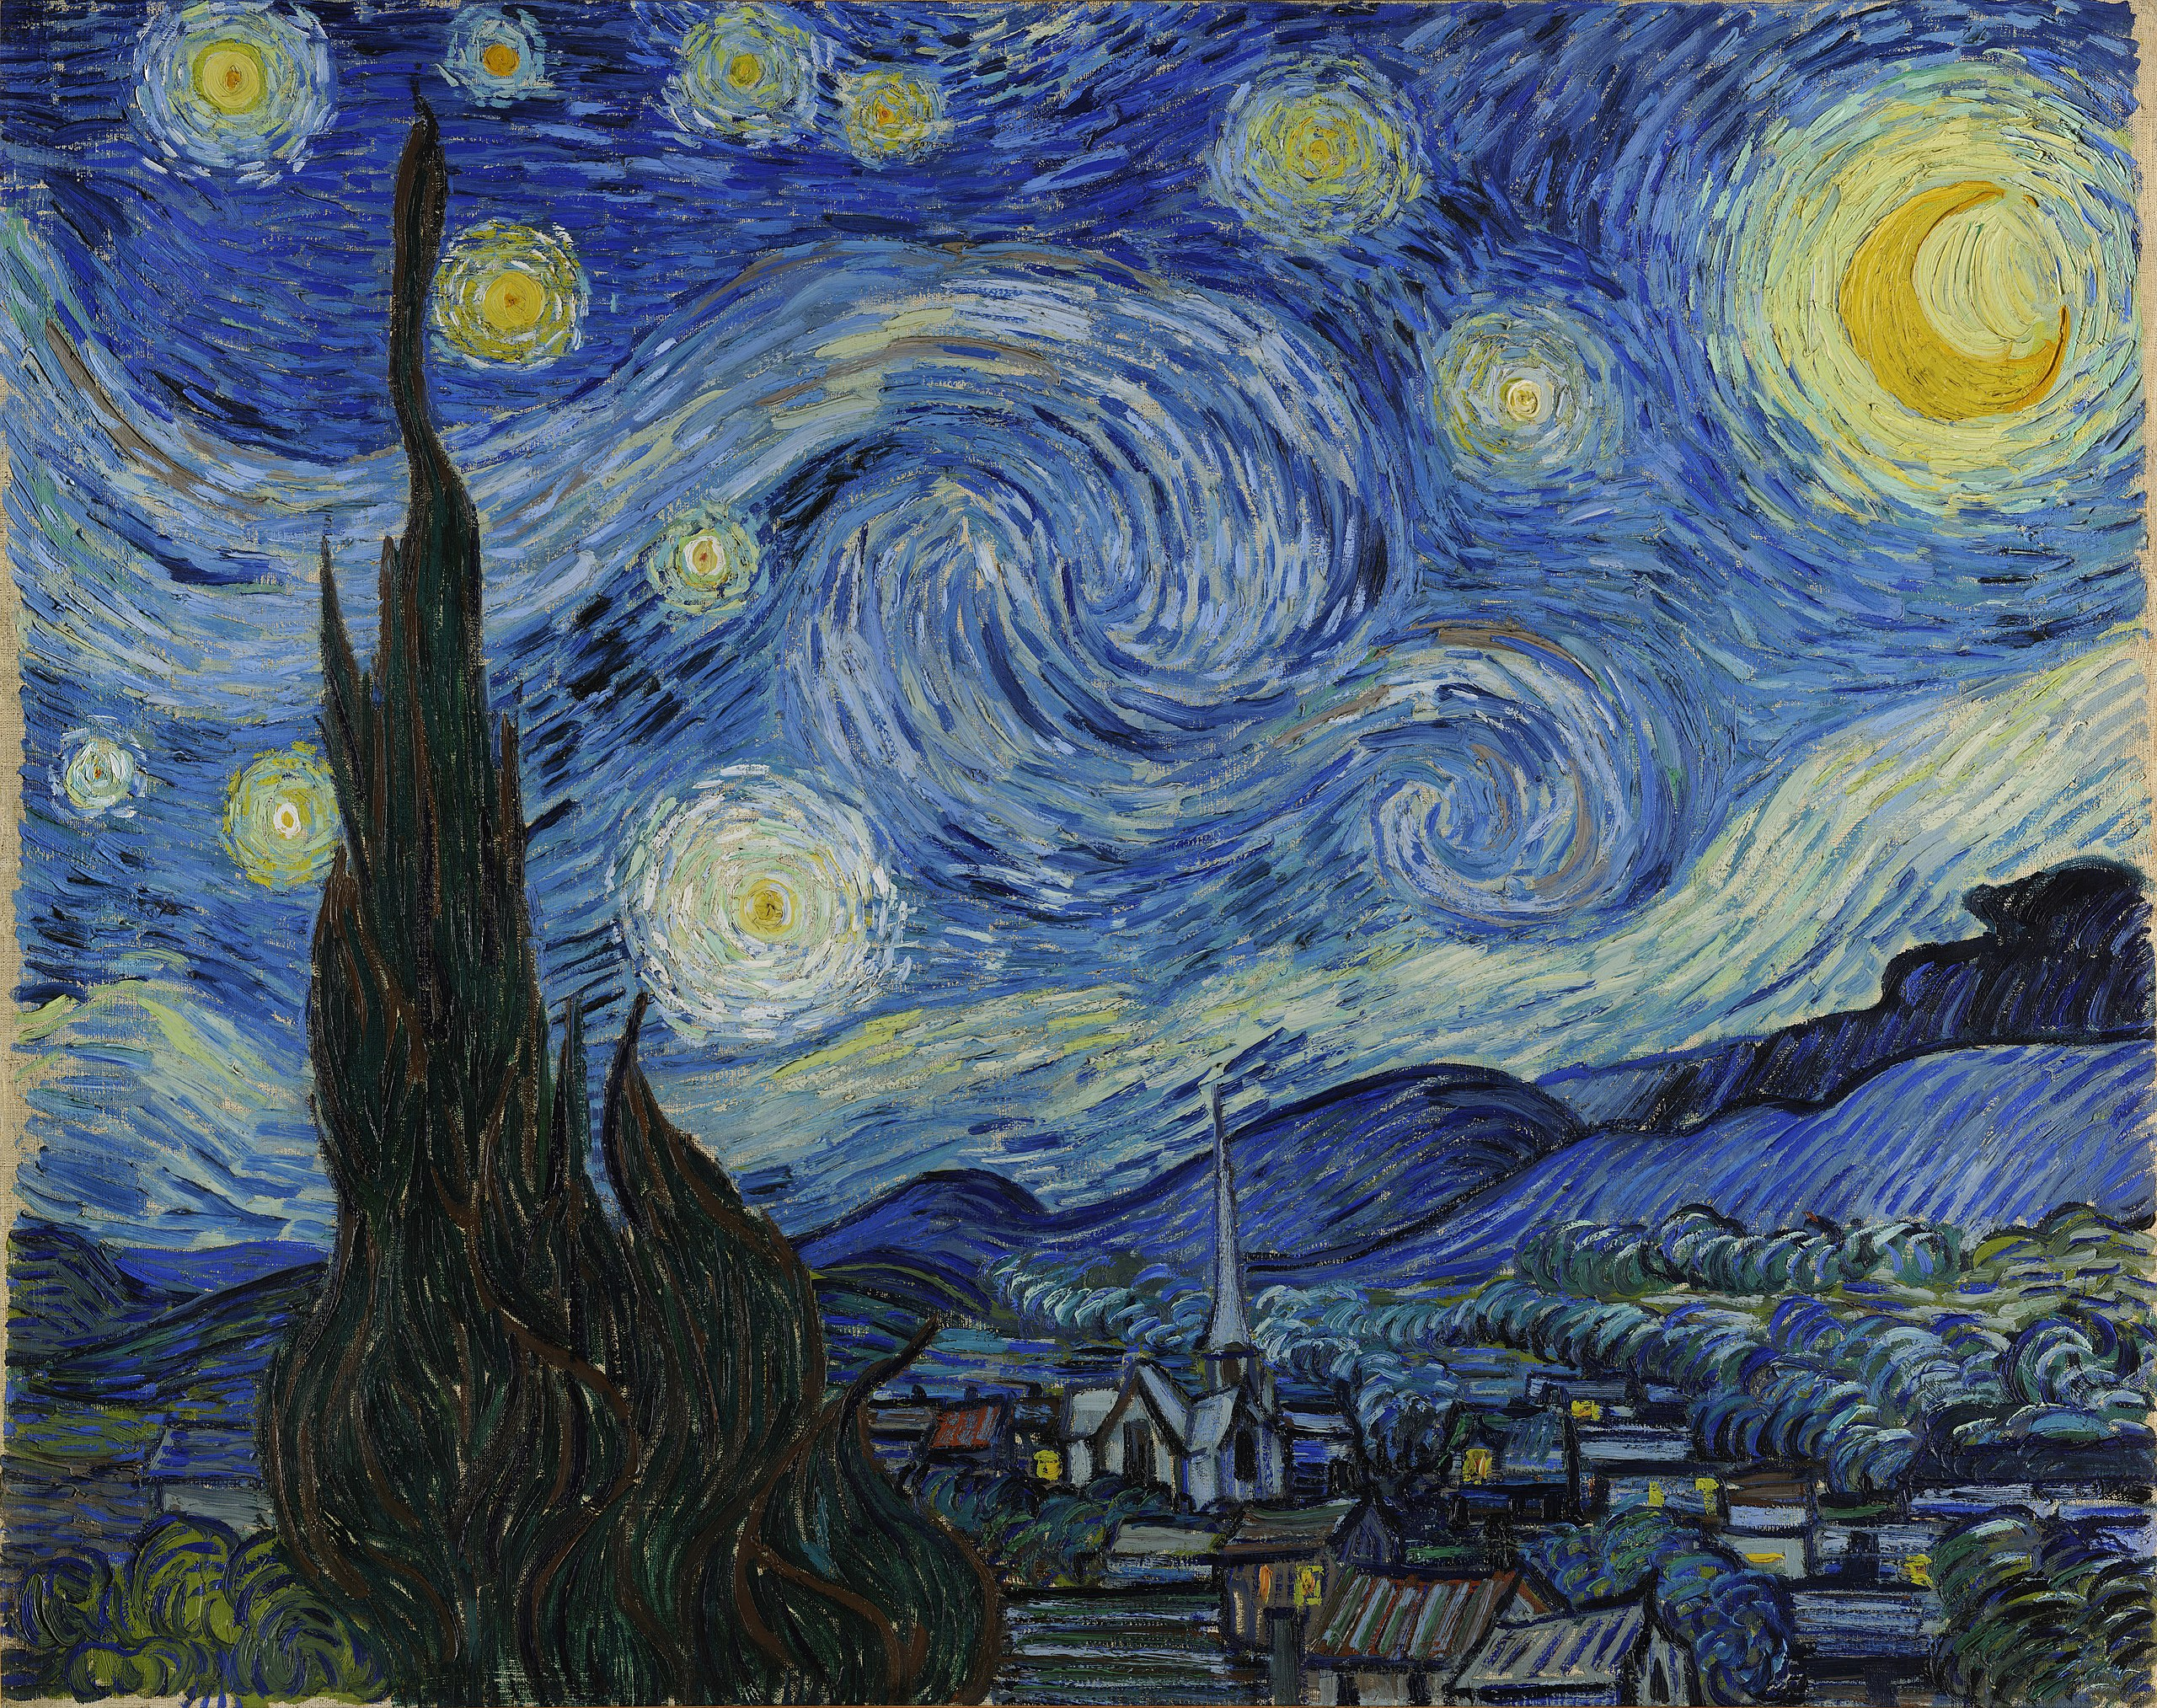
\includegraphics{figures/paintingexamples/starrynight}}
\caption{Like it or not, a continuous relation $[0,1] \rightarrow \blacksquare$: "The Starry Night", by Vincent van Gogh.}
\end{marginfigure}
\clearpage
\newpage
\section{Continuous Relations}

\newthought{To the best of my knowledge, the study of \textbf{TopRel} is a novel contribution. I venture two potential reasons.}

\newthought{First, it is because and not despite of the na\"{i}vity of the construction.} Usually, the relationship between \textbf{Rel} and \textbf{Set} is often understood in sophisticated general methods which are inappropriate in different ways. I have tried applying Kliesli machinery which generalises to "relationification" of arbitrary categories via appropriate analogs of the powerset monad to relate \textbf{Top} and \textbf{TopRel}, but it is not evident to me whether there is such a monad. The view of relations as spans of maps in the base category should work, since \textbf{Top} has pullbacks, but this makes calculation difficult and especially cumbersome when monoidal structure is involved. The na\"{i}ve approach I take is to observe that the preimages of functions are precisely relational converses when functions are viewed as relations, so the preimage-preserves-opens condition that defines continuous functions directly translates to the relational case.

\newthought{Second, the relational nature of \textbf{TopRel} means that the category has poor exactness properties.} Even if the sophisticated machinery mentioned in the first reason do manage to work, relational variants of \textbf{Top} are poor candidates for any kind of serious mathematics because they lack many limits and colimits. Since we take an entirely "monoidal" approach -- a relative newcomer in terms of mathematical technique -- we are able to find and make use of the rich structure of \textbf{TopRel} with a different toolkit.\\

In the end, we want to formalise doodles, so perhaps there is some virtue in proceeding by elementary means.

\marginnote{
\begin{rem}[Topological Space]
A \emph{topological space} is a pair $(X,\tau)$, where $X$ is a set, and $\tau \subset \mathcal{P}(X)$ are the \emph{open sets} of $X$, such that:
\begin{description}
    \item["nothing" and "everything" are open]  \[\varnothing,X \in \tau\]
    \item[Arbitrary unions of opens are open] \[\{ U_i : i \in I \} \subseteq \tau \Rightarrow \bigcup\limits_{i \in I} U_i \in \tau \]
    \item[Finite intersections of opens are open] $n \in \mathbb{N}$: \[U_1,\cdots, U_n \in \tau \Rightarrow \bigcap\limits_{1\cdots, i , \cdots n} U_i \in \tau\]
\end{description}
\end{rem}
}

\marginnote{
\begin{rem}[Relational Converse]
Recall that a relation $R: S \rightarrow T$ is a subset $R \subseteq S \times T$. \[R^\dag : T \rightarrow S := \{ (t,s) : (s,t) \in R \}\]
\end{rem}
}

\marginnote{
\begin{rem}[Continuous function]
A function between sets $f: X \rightarrow Y$ is a continuous function between topologies $f: (X,\tau) \rightarrow (Y,\sigma)$ if \[U \in \sigma \Rightarrow f^{-1}(U) \in \tau\] where $f^{-1}$ denotes the inverse image.
\end{rem}
}

Recall that functions are relations, and the inverse image used in the definition of continuous maps is equivalent to the relational converse when functions are viewed as relations. So we can na\"{i}vely extend the notion of continuous maps to continuous relations between topological spaces.

\begin{defn}[Continuous Relation]\label{defn:toprelation}
A continuous relation $R: (X,\tau) \rightarrow (Y,\sigma)$ is a relation $R: X \rightarrow Y$ such that \[U \in \sigma \Rightarrow R^{\dag}(U) \in \tau\] where $\dag$ denotes the relational converse.
\end{defn}

\begin{notation}
For shorthand, we denote the topology $(X,\tau)$ as $X^{\tau}$. As special cases, we denote the discrete topology on $X$ as $X^{\star}$, and the indiscrete topology $X^{\circ}$.
\end{notation}

The symmetric monoidal structure is that of product topologies on objects, and products of relations on morphisms.

\marginnote{
\begin{rem}[Product Topology]
We denote the product topology of $X^\tau$ and $Y^\sigma$ as $(X \times Y)^{(\tau \times \sigma)}$. $\tau \times \sigma$ is the topology on $X \times Y$ generated by the basis $\{t \times s : t \in \mathfrak{b}_\tau, s \in \mathfrak{b}_\sigma\}$, where $\mathfrak{b}_\tau$ and $\mathfrak{b}_\sigma$ are bases for $\tau$ and $\sigma$ respectively.
\end{rem}
}

\marginnote{
    \begin{rem}[Product of relations]
    For relations between sets $R: X \rightarrow Y, S: A \rightarrow B$, the product relation $R \times S: X \times A \rightarrow Y \times B$ is defined to be \[ \{ ((x,a),(y,b)) : (x,y) \in R, (a,b) \in S \} \]
    \end{rem}
}

\begin{fullwidth}

\section{\textbf{TopRel} diagrammatically}

\subsection{Relations that are always continuous}

\newthought{Here are five continuous relations for any $X^\tau$:}

\[\scalebox{0.75}{\tikzfig{bestiary/generators}}\]

\newthought{Copy and delete obey the following equalities:}

\[\scalebox{0.75}{\tikzfig{bestiary/basicrelations}}\]

\newthought{The copy map can also be used to distinguish the deterministic maps -- points and functions -- which we notate with an extra dot.}

\[\scalebox{0.75}{\tikzfig{structure/determinism}}\]

\newthought{Everything, delete, nothing-states and nothing-tests combine to give two numbers, one and zero.} There are extra expressions in grey squares above: they anticipate the tape-diagrams we will later use to graphically express another monoidal product of \textbf{TopRel}, the direct sum $\oplus$.

\[\scalebox{0.75}{\tikzfig{bestiary/scalarrelations}}\]

\newthought{Zero scalars turn entire diagrams into zero morphisms.} There is a zero-morphism for every input-output pair of objects in \textbf{TopRel}. 

\[\scalebox{0.75}{\tikzfig{bestiary/zerorelations}}\]

\end{fullwidth}
\clearpage
\newpage
\section{Populating space with shapes using sticky spiders}\label{sec:stickyspider}

%\begin{figure}\label{fig:spiderbicate}
%\scalebox{0.7}{\tikzfig{bestiary/spiderbicat}}
%\caption{The generators (in dashed boxes) and relations that make a spider. When the spider satisfies in addition the three inequalities b1-3, we call it a \textbf{relation-spider}.}
%\end{figure}

In this section, we seek to process-theoretically characterise disjoint collections of open sets of a space, so that we can play with doodles on the page as formal objects. It turns out that in \textbf{ContRel}, we can express them as idempotents that interact with spiders in a certain way.

\begin{example}[The copy-compare spiders of $\mathbf{Rel}$ are not always continuous]\label{ex:compnotspider}
The compare map for the Sierpi\'{n}ski space is not continuous, because the preimage of $\{0,1\}$ is $\{(0,0),(1,1)\}$, which is not open in the product space of $\mathcal{S}$ with itself.
\end{example}

\begin{rem}[copy-compare spiders of $\mathbf{Rel}$]
For a set $X$, the \emph{copy} map $X \rightarrow X \times X$ is defined:
\[\{(x,(x,x)) : x \in X \}\]
the \emph{compare} map $X \times X \rightarrow X$ is defined:
\[\{((x,x),x) : x \in X \}\]
These two maps are the (co)multiplications of special frobenius algebras. The (co)units are \emph{delete}:
\[\{(x,\star) : x \in X\}\]
and \emph{everything}:
\[\{(\star,x) : x \in X\}\]
\end{rem}

\newpage

\begin{myboxR}
\begin{proposition}\label{prop:copydiscrete}
The copy map is part of a special commutative frobenius algebra iff the topology is discrete.
\begin{proof}
Discrete topologies inherit the usual copy-compare spiders from \textbf{Rel}, so we have to show that when the copy map is part of a spider, the underlying wire must have a discrete topology. Suppose that some wire has a spider, and construct the following open set using an arbitrary point $p$:
\[\scalebox{0.5}{\tikzfig{structure/copyspiderproof/openpoint}}\]
It will suffice to show that this open set tests whether the input is the singleton $\{p\}$ -- when all singletons are open, the topology is discrete. As a lemma, we show that comparing distinct points $p \neq q$ yields the empty state.
\[\scalebox{0.5}{\tikzfig{structure/copyspiderproof/openpointproof}}\]
The (zero) implication follows since $p \neq q$ by assumption, so we know that deleting the comparison of $p$ and $q$ cannot be the unit scalar, and so must be the zero scalar, hence the comparison of $p$ and $q$ is the empty state. Now, the following case analysis shows that our open set only contains the point $p$.
\[\resizebox{0.75\textwidth}{!}{\tikzfig{structure/copyspiderproof/openpointcases}}\]
\end{proof}
\end{proposition}
\end{myboxR}

\begin{myboxB}
\begin{defn}[Sticky spiders]\label{defn:stickyspider}
A \textbf{sticky spider} (or just an $e$-spider, if we know that $e$ is a split idempotent), is a spider \emph{except} every identity wire on any side of an equation is replaced by the idempotent $e$.
\end{defn}

The desired graphical behaviour of a sticky spider is that one can still coalesce all connected spider-bodies together, but the 1-1 spider "sticks around" rather than disappearing as the identity. This is achieved by the following rules that cohere the idempotent $e$ with the (co)unit and (co)multiplications; they are the same as the usual rules for a special commutative frobenius algebra with two exceptions. First, where an identity wire appears in an equation, we replace it with an idempotent. Second, the monoid and comonoid components freely emit and absorb idempotents. By these rules, the usual proof [] for the normal form of spiders follows, except the idempotent becomes an explicit 1-1 spider, rather than the identity.
\[\resizebox{\textwidth}{!}{\tikzfig{structure/idemspider/stickyrelations}}\]
\end{myboxB}

\begin{myboxR}
\newthought{We can use split idempotents to transform copy-spiders from discrete topologies to sticky-spiders on other spaces.}
\begin{rem}[Split idempotents]
An \textbf{idempotent} in a category is a map $e: A \rightarrow A$ such that \[A \overset{e}{\rightarrow} A \overset{e}{\rightarrow} A = A \overset{e}{\rightarrow} A\]
A \textbf{split idempotent} is an idempotent $e: A \rightarrow A$ along with a \textbf{retract} $r: A \rightarrow B$ and a \textbf{section} $s: B \rightarrow A$ such that:
\[A \overset{e}{\rightarrow} A = A \overset{r}{\rightarrow} B \overset{s}{\rightarrow} A\]
\[B \overset{s}{\rightarrow} A \overset{r}{\rightarrow} B = B \overset{\mathop{id}}{\rightarrow} B\]
\end{rem}

We can graphically express the behaviour of a split idempotent $e$ as follows, where the semicircles for the section and retract $r,s$ form a visual pun. Recall that $X^\star$ denotes the discrete topology on the set $X$.

\[\scalebox{1}{\tikzfig{structure/idemspider/splitidem}}\]
\end{myboxR}

\begin{myboxB}
\begin{construction}[Sticky spiders from split idempotents]\label{cons:stickyfromsplit}
Given an idempotent $e: Y^\sigma \rightarrow Y^\sigma$ that splits through a discrete topology $X^\star$, we construct a new (co)multiplication as follows:
\[\scalebox{1}{\tikzfig{structure/idemspider/idemspiderv2}}\]
\end{construction}
\end{myboxB}

\begin{myboxR}
\begin{proposition}[Every idempotent that splits through a discrete topology gives a sticky spider]\label{prop:splitmeanssticky} The following is a sticky spider:
\[\scalebox{1}{\tikzfig{structure/idemspider/espiderstatement}}\]
\end{proposition}
We can check that Construction \ref{cons:stickyfromsplit} satisfies the frobenius rules as follows. We only present one equality; the rest follow the same idea.
\[\scalebox{1}{\tikzfig{structure/idemspider/espiderproofv2}}\]
\end{myboxR}
\begin{myboxR}
To verify the sticky spider rules, we first observe that since $X^\star \overset{s}{\rightarrow} Y^\sigma \overset{r}{\rightarrow} X^\star = X^\star \overset{\mathop{id}}{\rightarrow} X^\star$, $r$ must have all of $X^\star$ in its image, and $s$ must have all of $X^\star$ in its preimage, so we have the following:
\[\scalebox{1}{\tikzfig{structure/idemspider/splitonto}}\]
Now we show that e-unitality holds:
\[\scalebox{1}{\tikzfig{structure/idemspider/espiderproof2}}\]
The proofs of e-counitality, and e-speciality follow similarly.
\end{myboxR}

\begin{myboxB}
\newthought{We can prove a partial converse of Proposition \ref{prop:splitmeanssticky}:} we can identify two diagrammatic equations that tell us precisely when a sticky spider has an idempotent that splits though some discrete topology.
\begin{theorem}\label{thm:stickygraphical}
A sticky spider has an idempotent that splits through a discrete topology if and only if in addition to the sticky spider equalities, the following relations are also satisfied.
\[\scalebox{1}{\tikzfig{idemproof/unit-everything}} \quad\quad\quad\quad\quad\quad\quad\quad \scalebox{1}{\tikzfig{idemproof/comult-copy}}\]
\end{theorem}
The proof is involved, so here is a map of lemmas and propositions.
\[\resizebox{0.8\textwidth}{!}{\tikzfig{idemproof/claimmap2}}\]
\end{myboxB}

\begin{myboxR}
\begin{proposition}[comult/copy implies counit/delete]\label{prop:counitdelete}
\[\scalebox{1}{\tikzfig{idemproof/ecopy2delclaim}}\]
\begin{proof}
\[\scalebox{1}{\tikzfig{idemproof/ecopy2del}}\]
\end{proof}
\end{proposition}
\end{myboxR}

\begin{myboxB}
\begin{lemma}[All-or-Nothing]\label{lem:allornothing}
Consider the set $e(\{x\})$ obtained by applying the idempotent $e$ to a singleton $\{x\}$, and take an arbitrary element $y \in e(x)$ of this set. Then $e(\{y\}) = \varnothing$ or $e(\{x\}) = e(\{y\})$. Diagrammatically: \[\scalebox{0.75}{\tikzfig{idemproof/allornothingclaim}}\]
\end{lemma}
\[\scalebox{0.75}{\tikzfig{idemproof/allornothing2a}}\]
\end{myboxB}
\begin{myboxB}
\[\scalebox{0.75}{\tikzfig{idemproof/allornothing2b}}\]
\end{myboxB}

\begin{myboxR}
\begin{proposition}[$e$ of any point is $e$-copiable]\label{prop:epointcopy}
\[\scalebox{0.75}{\tikzfig{idemproof/pointidemcopiable}}\]
\begin{proof}
\[\scalebox{0.75}{\tikzfig{idemproof/pointidemcopiableproof}}\]
\end{proof}
\end{proposition}
\end{myboxR}

\begin{myboxB}
\begin{proposition}[The unit is the union of all $e$-copiables]\label{prop:copiablebasis}
\[\scalebox{0.8}{\tikzfig{idemproof/copiablebasisclaim}}\]
\begin{proof}
\[\scalebox{0.8}{\tikzfig{idemproof/copiablebasis}}\]
\end{proof}
\end{proposition}
\end{myboxB}

\begin{myboxR}
\begin{proposition}[$e$-copiable decomposition of $e$]\label{prop:decompidem}
\[\scalebox{1}{\tikzfig{idemproof/decompidemclaim}}\]
\begin{proof}
\[\scalebox{1}{\tikzfig{idemproof/decompidem}}\]
\end{proof}
\end{proposition}
\end{myboxR}

\begin{myboxB}
\begin{proposition}[$e$-copiable decomposition of counit]\label{prop:decompcounit}
\[\scalebox{1}{\tikzfig{idemproof/decompcounitclaim}}\]
\begin{proof}
\[\scalebox{1}{\tikzfig{idemproof/decompcounit}}\]
\end{proof}
\end{proposition}
\end{myboxB}

\begin{myboxR}
\newthought{The $e$-copiable states really do behave like an orthonormal basis, as the following Lemmas show.}
\begin{lemma}[$e$-copiables are orthogonal under multiplication]\label{lem:match}
\[\scalebox{0.75}{\tikzfig{idemproof/matchclaim}}\]
\begin{proof}
\[\scalebox{0.75}{\tikzfig{idemproof/match}}\]
\end{proof}
\end{lemma}
\end{myboxR}

\begin{myboxB}
\begin{convention}[Shorthand for the open set associated with an $e$-copiable]
We introduce the following diagrammatic shorthand.
\[\scalebox{1}{\tikzfig{idemproof/openshorthand}}\]
Including the coloured dot is justified, because these open sets are co-copiable with respect to the multiplication of the sticky spider.
\[\scalebox{1}{\tikzfig{idemproof/shorthandjustification}}\]
\end{convention}
\end{myboxB}

\begin{myboxR}
\begin{lemma}[Co-match]\label{lem:comatch}
\[\scalebox{1}{\tikzfig{idemproof/comatchclaim}}\]
\begin{proof}
\[\scalebox{0.9}{\tikzfig{idemproof/comatch}}\]
The claim then follows by applying Lemma \ref{lem:match} to the final diagram.
\end{proof}
\end{lemma}
\end{myboxR}

\begin{myboxB}
\begin{lemma}[e-copiables are e-fixpoints]\label{lem:ecopyfixpoint}
\[\scalebox{1}{\tikzfig{idemproof/dotcopyableclaim}}\]
\begin{proof}
\[\scalebox{1}{\tikzfig{idemproof/dotcopyable}}\]
Observe that the final equation of the proof also holds when the initial e-copiable is the empty set.
\end{proof}
\end{lemma}
\end{myboxB}

\begin{myboxR}
\begin{lemma}[$e$-copiables are normal]\label{lem:ecopynormal}
\[\scalebox{1}{\tikzfig{idemproof/copynormalclaim}}\]
\begin{proof}
\[\scalebox{1}{\tikzfig{idemproof/copynormal}}\]
\end{proof}
\end{lemma}
\end{myboxR}

\begin{myboxB}
\begin{proposition}[$e$-copiable decomposition of multiplication]\label{prop:decompmult}
\[\scalebox{1}{\tikzfig{idemproof/decompmultclaim}}\]
\begin{proof}
\[\scalebox{1}{\tikzfig{idemproof/decompmult}}\]
\end{proof}
\end{proposition}
\end{myboxB}

\begin{myboxR}
\begin{proposition}[$e$-copiable decomposition of comultiplication]\label{prop:decompcomult}
\[\scalebox{1}{\tikzfig{idemproof/decompcomultclaim}}\]
\begin{proof}
\[\scalebox{1}{\tikzfig{idemproof/decompcomult}}\]
\end{proof}
\end{proposition}
\end{myboxR}

\begin{myboxB}
\newthought{Now we can prove Theorem \ref{thm:stickygraphical}.}
First a reminder of the claim; we want to show that when given a sticky spider, the following relations hold if and only if the idempotent splits through a discrete topology.
\[\scalebox{0.8}{\tikzfig{idemproof/unit-everything}} \quad\quad\quad\quad\quad\quad\quad\quad \scalebox{0.8}{\tikzfig{idemproof/comult-copy}}\]
The crucial observation is that the $e$-copiable decomposition of the idempotent given by Proposition \ref{prop:decompidem} is equivalent to a split idempotent though the set of $e$-copiables equipped with discrete topology.
\[\scalebox{0.8}{\tikzfig{idemproof/finalproof}}\]
By copiable basis Proposition \ref{prop:copiablebasis} and the decompositions Propositions \ref{prop:decompcounit}, \ref{prop:decompmult}, \ref{prop:decompcomult}, we obtain the only-if direction.
\[\scalebox{0.8}{\tikzfig{idemproof/finalproof2}}\]
\end{myboxB}
\begin{myboxB}
The if direction is an easy check. For the unit/everything relation, we have:
\[\scalebox{0.8}{\tikzfig{idemproof/finalproof3}}\]
For the counit/delete relation, we observe that for any split idempotent, the retract must be a partial function. To see this, suppose the split idempotent $e = r;s$ is on $(X,\tau)$ and the discrete topology is $Y^\star$. Seeking contradiction, if the retract is not a partial function, then there is some point $x \in X$ such that $x \in e(x)$, and the image $I := r(x) \subseteq Y$ contains more than one point, which we denote and discriminate $a,b \in r(x) \subseteq Y$ and $a \neq b$. Because the composite $s;r = 1_Y$ of the section and retract must recover the identity on $Y^\star$, the section $s$ must be total -- i.e. the image $s(X) = Y$. So $x \in s(a) \cap s(b)$. Now we have that $(a,x),(b,x) \in s$, and $(x,a),(x,b) \in r$, therefore $(a,b),(b,a) \in s;r$, which by $a \neq b$ contradicts that $s;r$ is the identity relation $1_Y$.
\[\scalebox{0.8}{\tikzfig{idemproof/finalproof4}}\]
\end{myboxB}

\begin{myboxR}
\begin{defn}[Labels, shapes, cores, halos]
Recall by Proposition \ref{prop:decompidem} that we can express the idempotent as a union of continuous relations formed of a state and test, for some indexing set of \emph{labels} $\mathcal{L}$.
\[\tikzfig{topology/shape1}\]
A \emph{shape} is a component of this union corresponding to some arbitary $l \in L$. So we refer to a sticky spider as a labelled collection of shapes. The state of a shape is the \emph{halo} of the shape. The halos are precisely the copiables of the sticky spider. The test of a shape is the \emph{core}. The cores are precisely the cocopiables of the sticky spider.
\[\tikzfig{topology/shape2}\]
\end{defn}
\end{myboxR}

\begin{myboxB}
\begin{proposition}[Core exclusion: Distinct cores cannot overlap]\label{prop:core-core-exclusion}
\begin{proof}
A direct consequence of Lemma \ref{lem:comatch}.
\end{proof}
\end{proposition}
\end{myboxB}

\begin{myboxR}
\begin{proposition}[Core-halo exclusion: Each core only overlaps with its corresponding halo]\label{prop:core-halo-exclusion}
\begin{proof}
Seeking contradiction, if a core overlapped with multiple halos, Lemma \ref{lem:ecopyfixpoint} would be violated.
\end{proof}
\end{proposition}
\end{myboxR}

\begin{myboxB}
\begin{proposition}[Halo non-exclusion: halos may overlap]
\begin{proof}
By example:
\[\tikzfig{topology/halooverlap}\]
The two shapes are colour coded cyan and magenta. The halos are two triangles which overlap at a yellow region, and partially overlap with their blobby cores. The cores are outlined in dotted blue and orange respectively. Observe that cores and halos do not have to be simply connected; in this example the core of the magenta shape has two connected components. Viewing these sticky spiders as a process, any shape that overlaps with the magenta core will be deleted and replaced by the magenta triangle, and similarly with the cyan cores and triangle. Any shape that overlaps with both the magenta and cyan cores will be deleted and replaced by the union of the triangles. Any shape that overlaps with neither core will be deleted and not replaced.
\end{proof}
\end{proposition}
\end{myboxB}

\begin{myboxR}
\begin{corollary}[Only opens please]
A sticky spider corresponds to a set-indexed disjoint collection of open sets when, in addition to the equations of Theorem \ref{thm:stickygraphical}, it satisfies one more, depicted below on the left.
\[\scalebox{1}{\tikzfig{idemproof/opensonly}}\]
Observe that the right hand equation above is precisely what we want expressed in diagrams: that every halo matches its core. For the forward direction, we have:
\[\scalebox{1}{\tikzfig{idemproof/opensonly3}}\]
\end{corollary}
\end{myboxR}

\begin{myboxR}
For the backward direction, we rely on the fact that cores are non-empty (or else we would fail to satisfy the identity equation of the split idempotent) to eliminate the floating scalars.
\[\scalebox{1}{\tikzfig{idemproof/opensonly2}}\]
By Proposition \ref{prop:core-core-exclusion}, we have disjointness.\\

So, without loss of generality, we may treat any collection of disjoint open shapes on a page as a sticky spider.
\end{myboxR}

\clearpage
%clearpage
%newpage
%input{chapters/sketches/prelims}
%clearpage
%newpage
%input{chapters/sketches/temporal}
%clearpage
%newpage
%input{chapters/sketches/modals}
%clearpage
%newpage
%input{chapters/sketches/turing}
%clearpage
%newpage
%input{chapters/sketches/config}
%clearpage
%newpage
%input{chapters/beyond/metaphor}

\bibliographystyle{alpha}
\bibliography{thesis_intro}






\end{document}